	\subsection{Индекс Эрбана}

	Пусть $G$ конечная группа и предположим дополнительно, что 
	\[
		|\widehat{H}^0(G, A)| < \infty, \quad |\widehat{H}^1(G, A)| < \infty.
	\]
	\begin{remark}
		Позже мы увидим, что для конечных групп группы когомологий Тейта периодичны, так что это означает, что все когомологии конечны. 
	\end{remark}

	\begin{definition} 
		Пусть $A \in G\text{-}\Mod$. Его \emph{индексом Эрбана} мы будем называть  
		\[
			h(A) = \frac{|\widehat{H}^0(G, A)|}{|\widehat{H}^1(G, A)|}.
		\]
	\end{definition}

	Докажем лемму, которая помогает удобно вычислять индекс Эрбана. 

	\begin{statement}\label{Herbran_calculation} 
		Пусть $G$~--- конечная  циклическая группа, а $0 \to A \to B \to C \to 0$~--- короткая точная последовательность $\Z[G]$-модулей. Предположим, что два из трё индексов Эрбана $h(A), h(B), h(C)$ определены. Тогда определён и третий и, более того, 
		\[
			h(B) = h(C) \cdot h(A).
		\]
	\end{statement}
	\begin{proof}
		Так как группа циклическая (и её когомологии периодичны), из длинной точной последовательности пары мы получаем вот такой коммутативный шестиугольник (бензольное кольцо): 
		\begin{center}
			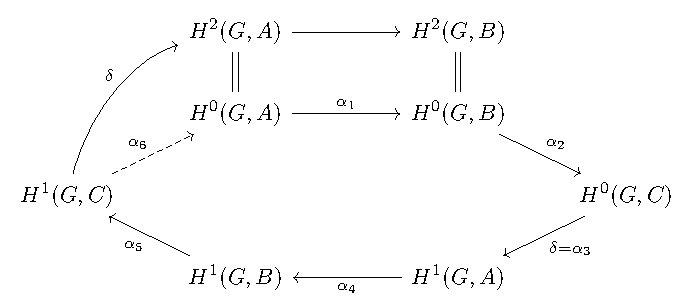
\includegraphics{lectures/6/pictures/cd_20.pdf}
		\end{center}

		Соответственно, обозначая $M_i = \ker{\alpha_i} = \Im_{\alpha_{i - 1}}$, мы получаем такие короткие точные последовательности: 
		\[
			\begin{cases} 0 \to M_1 \to H^0(G, A) \to M_2 \to 0  \\ 0 \to M_2 \to H^0(G, B) \to M_3 \to 0 \\ \vdots \\ 0 \to M_6 \to H^1(G, C) \to M_1 \to 0\end{cases} \implies h(A) = \frac{H^0(G, A)}{H^1(G, A)} = \frac{|M_1| \cdot ||M_2|}{|M_4| \cdot |M_5|}, \ 
		\]
		и, аналогичным образом: 
		\[
			h(B) = \frac{|M_2| \cdot |M_3|}{|M_5| \cdot |M_6|}, \quad h(C)  = \frac{|M_3| \cdot |M_4|}{|M_1| \cdot |M_6|}, 
		\]
		откуда $h(A) \cdot h(C) = h(B)$. 
	\end{proof}	

	\begin{corollary}\label{Herbran_index_of_finite_module}
		Пусть $G$~--- конечная циклическая группа, и при этом $G$-модуль $A$ конечный. Тогда $h(A) = 1$.
	\end{corollary}
	\begin{proof}
		Запишем две  точные последовательности: 
		\[
			0 \to \Ker{N} \to A \xrightarrow{\cdot N} \to A^{G} \to \widehat{H}^0(G, A) \to 0
		\]
		\[
			0 \to A^G \to A \xrightarrow{\cdot (\sigma - 1)} \Ker{N} \to H^{1}(G, A) \to 0.
		\]

		Тогда мы имеем 
		\[
			|\widehat{H}^0(G, A)| = \frac{|A^G| \cdot |\Ker{N}|}{|A|}, \quad |\widehat{H}^1(G, A)| = \frac{|A^G| \cdot |\ker{N}|}{|A|},
		\]
		откуда видно, что $h(A) = 1$. 
	\end{proof}

	\begin{corollary}
		Пусть $A, B \in G\text{-}\Mod$, $f \in \Hom_{G}(A, B)$ и при этом $|\ker{f}| < \infty$ и $|\Coker{f}| < \infty$. Тогда если один из индексов Эрбрана $h(A), h(B)$ определён, то они оба определены и совпадают.
	\end{corollary}
	\begin{proof}
		Теперь у нас есть такие короткие точные последовательности: 
		\[
			0 \to \Ker{f} \to A \twoheadrightarrow \Im{f} \to 0
		\]
		\[
			0 \to \Im{f} \to B \to \Coker{f} \to 0.
		\]
		Не умаляя общности, $h(A)$ определён. Тогда мы получаем, что 
		\[
			\begin{cases} h(A) \text{ определён } h(\ker{f}) = 1 \end{cases}   \implies h(\Im{f}) \text{ определён }.
		\]
		\[
			\begin{cases} h(\Coker{f}) = 1  \\ h(\Im{f}) \text{ определён } \end{cases} \implies h(b) \text{ определён }
		\]
		и, из формул выше следует, что $h(B) = h(\Im{f}) \cdot h(\Coker{f})$. Но тогда 
		\[
			h(B) = h(\Im{f}) = \frac{h(A)}{h(\ker{f})} = h(A). 
		\]
	\end{proof}


	\subsection{Ограничение и инфляция}

	 Пусть $\varphi\colon H \to G$~--- гомоморфизм групп, а $A \in G\text{-}\Mod$. Тогда $A$ естественно наделяется структурой $H$-модуля следующим образом: 
	 \[
	 	a \cdot h \eqdef \varphi(h) \cdot a. 
	 \]

	 Тогда у нас есть гомоморфизм $\varphi^*\colon \Z[H] \to \Z[G]$, так как групповое кольцо это функтор, а значит, есть и морфизм комплексов 

	 \begin{center}
	 	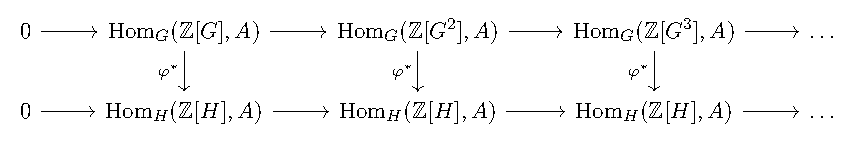
\includegraphics{lectures/6/pictures/cd_8.pdf}
	 \end{center}

	 и индуцированный морфизм на когомологиях $\varphi^*\colon H^k(G, A) \to H^k(H, A)$. 

	 \begin{definition} 
	 	Если $H \le G$ и $\varphi \colon H \hookrightarrow G$~--- это вложение, то индуцированный морфизм в когомологиях 
	 	\[
	 		H^{\bullet}(G, A) \xrightarrow{\res} H^{\bullet}(H, A)
	 	\]
	 	мы будем называть \emph{гомоморфизмом ограничения} и обозначать $\res$. 
	 \end{definition}

	 \begin{remark}
	 	Этот гомоморфизм, вообще говоря, не обязан быть мономорфизмом. 
	 \end{remark}


	 Пусть теперь $H \le G$~--- нормальная подгруппа, а $A \in G\text{-}\Mod$. Тогда $A^H$ можно естественным образом снабдить структурой $G/H$-модуля: 
	 \[
	 	(gh)a = ga.
	 \]
	 Соответственно, у нас есть диаграмма 
	 \begin{center}
	 	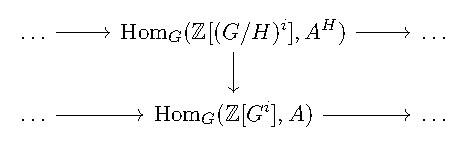
\includegraphics{lectures/6/pictures/cd_9.pdf}
	 \end{center}

	 \begin{definition} 
	 	Соответствующий индуцированный морфизм $H^{n}(G/H, A^H) \xrightarrow{\inf} H^n(G, A)$ в когомологиях мы будем называть \emph{инфляцией}.
	 \end{definition}

	 \begin{statement} 
	 	Пусть $A \in G\text{-}\Mod$, $H$~--- нормальная подгруппа в $G$. Тогда следующая последовательность точна: 
	 	\[
	 		0 \to H^{1}(G/H, A^H) \xrightarrow{\inf} H^1(G, A) \xrightarrow{\res} H^1(H, A).
	 	\]
	 \end{statement}
	 \begin{proof}
	 	\noindent\bf{Шаг 1.} Пусть $f \in Z^1(G/H, A^H)$, тогда $f$ удовлетворяет 
	 	\[
	 		f(\overline{g_1} \overline{g_2}) = \overline{g_1} f(\overline{g_2}) + f(\overline{g_1}). 
	 	\]

	 	Предположим, что отображение 
	 	\[
	 		\inf(f) \colon G \xrightarrow{\pi} G/H \xrightarrow{f} \to A^H \to A
	 	\]
	 	является кограницей (не умаляя общности, назовём его той же буквой), то есть, существует $a \in A$ такой, что $\forall g \in G \ f(\overline{g}) = ga - a$. Проверим, что в таком случае $a \in A^H$. 

	 	\[
	 		\begin{cases} f(\overline{gh}) = f(\overline{g}) = ga - a \\ f(\overline{gh}) = g h a - a \implies gha = ga \implies h a = a \implies a \in A^H. \end{cases}
	 	\]
	 	Значит, $f \in B^{1}(G/H, A^H)$, то есть  мы проверили инъективность стрелки $\inf$.

	 	\noindent\bf{Шаг 2.} Докажем, что $\res \circ \inf = 0$. Пусть $f \in Z^1(G/H, A^H)$. Рассмотрим 
	 	\[
	 		\res \circ \inf(f) = \widetilde{f}\colon H \to G \to G/H \xrightarrow{f} A^H \hookrightarrow A
	 	\]
	 	В самом деле, тогда 
	 	\[
	 		\widetilde{f}(h) = f(\overline{1}) = 0 \implies \res \circ \inf(f) = 0.
	 	\]

	 	\noindent\bf{Шаг 3.} Пусть теперь $f \in Z^1(G; A)$ и $f \in \ker{(\res)}$. То есть, 
	 	\[
	 		f(g_1 g_2) = g_1 f(g_2) + f(g_1), \quad \exists a \colon f(h) = ha - a.
	 	\]
	 	Рассмотрим кограницу $\ell(g) = ga - a \in B^{1}(G, A)$. Тогда $[f] = [f - \ell]$, но 
	 	\[
	 		(f - \ell)(h) = ha - a - (ha - a) = 0, 
	 	\]
	 	поэтому мы с самого начала можем полагать, что наш представитель $f\vert_{H} \equiv 0$. Тогда можно попустить отображение через фактор: 

	 	\begin{center}
	 		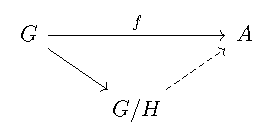
\includegraphics{lectures/6/pictures/cd_10.pdf}
	 	\end{center}

	 	С другой же стороны, 
	 	\[
	 		f(h g_2) = h f(g_2) + f(h) = h f(g_2),
	 	\]
	 	откуда ясно, что отображение пропускается через $A^H$, т.е. у нас есть вот такая диаграмма 
	 	\begin{center}
	 		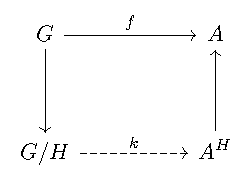
\includegraphics{lectures/6/pictures/cd_11.pdf}
	 	\end{center}
	 	и очевидно, что $k$~--- коцикл. 
	 \end{proof}

	 Теперь распространим гомоморфизм ограничения на отрицательные размерности. 


	 Пусть $A$~--- $G$-модуль, $H \hookrightarrow$, тогда есть отображение $A^{G} \hookrightarrow A^{H}$ (действительно, если $a \in A$ неподвижен под действием всех элементов из $G$, то под действием всех элементов из $H$ уж точно). Тогда есть и корректное отображение 
	 \[
	 	A^{G}/N_{G}A \to A^{H}/N_{H}A.
	 \]
	 В самом деле, если $x \in N_{G}A$, то $x = \sum_{\sigma} \sigma \cdot a$ для некоторого $a$. Заметим, что 
	 \[
	 	G = \bigsqcup_{i} \sigma_i H.
	 \]
	 Соответственно, тогда мы имеем
	 \[
	 	N_{G}a = \sum_{\sigma \in G} \sigma a = \sum_{\tau \in H}\lr*{\sum_{i}\sigma_i a} = N_{H}\lr*{\sum_{i}\sigma_i a} \in N_H A.
	 \]

	 Таким образом мы смогли доопределить ограничение на нулевые когомологии Тейта: 
	 \[
	 	\res\colon \widehat{H}^0(G,A) \to \widehat{H}^0(H, A). 
	 \]
	 Осталось распространить его на отрицательные размерности. Рассмотрим короткую точную последовательность 
	 \[
	 	0 \to A'' \to A_{*} \to A \xrightarrow{\varphi} 0, \text{ где } A_* = \Z[G] \otimes_{Z} A,
	 \]
	 гомоморфизм $\varphi$ действует как $\sigma \otimes a \mapsto a$, а $A'' = \ker{\varphi}$. Так как модуль $A_*$ когомологически тривиален, то есть $\widehat{H}^n(G, A_*) = 0 \ \forall n \in \N$, мы получаем из длинной точной последовательности мы получаем следующую диаграмму (точнее говоря, горизонтальные изоморфимзы в ней) 

	 \begin{center}
	 	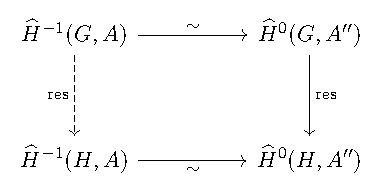
\includegraphics{lectures/6/pictures/cd_12.pdf}
	 \end{center}
	 
	 Тогда определим $\res$ в $-1$-й размерности, как пунктирную стрелочку, замыкающую диаграмму. 

	 \begin{remark}
	 	Вообще говоря, чтоб был у нас был изоморфизм когомологий Тейта для подгруппы $H$, нужно, чтоб $A_*$ был не только $G$-индуцированным, но и $H$-индуцированным. \textcolor{red}{Соответственно, надо проверить, почему же это так}. 
	 \end{remark}

    \subsection{Точная последовательность для ограничения и инфляции в старших размерностях}

	  Как мы видели ранее, если $A \in G\text{-}\Mod$, а $H$~--- нормальная подгруппа в $G$, то следующая последовательность точна: 
	 	\[
	 		0 \to H^{1}(G/H, A^H) \xrightarrow{\inf} H^1(G, A) \xrightarrow{\res} H^1(H, A).
	 	\]

	 В этом параграфе мы понятным образом обобщим этот результат на старшие размерности. 

	 \begin{statement} 
	 	Пусть $H \le G$~--- нормальная подгруппа, $A \in G\text{-}\Mod$, а кроме того 
	 	\[
	 		H^1(H, A) = H^2(H, A) = \ldots = H^{q - 1}(H, A) = 0.
	 	\]
	 	Тогда следующая последовательность точна: 
	 	\[
	 		0 \to H^{q}(G/H, A^H) \xrightarrow{\inf} H^q(G, A) \xrightarrow{\res} H^q(H, A).
	 	\]
	 \end{statement}
	 \begin{proof}
	 	Естественно, будем доказывать утверждение индукцией по $q$. 

	 	\noindent\bf{База:} Для $q = 1$ утверждение мы знаем. 

	 	\noindent\bf{Переход:} Рассмотрим короткую точную последовательность 
	 	\[
	 		0 \to A \to A^* \to A' \to 0,
	 	\]
	 	она индуцирует длинную точную последовательность когомологий: 
	 	\[
	 		0 \to A^H \to (A^*)^H \to (A')^H \to \underbrace{H^1(H, A)}_{= 0} \to \ldots	
	 	\]
	 	Из неё (так как $A^*$ коиндуцированный) мы получаем, что $H^{i}(H, A') \cong H^{i + 1}(H, A)$. Кроме того, из этой же короткой точной последовательности мы стандартным образом получаем, что $H^{q - 1}(G, A') \cong H^{q}(G, A)$.

	 	Обозначим для простоты $F = G/H$. Теперь заметим, что в частности из длинной точной последовательности сверху можно достать короткую точную последовательность
	 	\[
	 		0 \to A^H \to (A^*)^H \to (A')^H \to 0,
	 	\]
	 	как начальный кусок. Напишем длинную точную последовательность когомологий и для неё: 
	 	\[
	 		\ldots H^{q - 1}(F, \lr*{A^*}^H) \to H^{q - 1}(F, (A')^H) \to H^{q}(F, A^H) \to H^q(F, \lr*{A^*}^H) \to \ldots.
	 	\]
	 	Заметим, что $\lr*{A^*}^H = \Hom(\Z[G], A)^H \cong \Hom(\Z[G/H], A)$, откуда следует, что $\lr*{A^*}^H$~--- $H$-коиндуцированный модуль. Значит, из длинной точной последовательности выше мы заключаем, что 
	 	\[
	 		H^{q - 1}(F, (A')^H) \cong H^q(F, A^H).	
	 	\]

	 	Соответственно, тогда у нас есть такая коммутативная диаграмма: 

	 	\begin{center}
	 		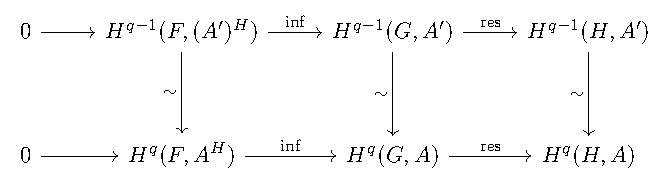
\includegraphics{lectures/6/pictures/cd_26.pdf}
	 	\end{center}
	 	Верхняя строка точна по индукционном предположению, а вертикальные стрелки~--- изоморфизмы. Значит, и нижняя строка точна. 
	 \end{proof}

	 \subsection{Отображение коограничения}

	 \begin{definition} 
	 	Пусть $H \le G$, тогда вложение $H \hookrightarrow G$ индуцирует морфизм цепных комплексов 

	 \begin{center}
	 	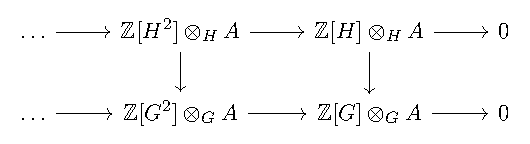
\includegraphics{lectures/6/pictures/cd_13.pdf}
	 \end{center}

	 Это цепное отображение индуцирует отображение в когомологиях $H_{n}(H, A) \to H_{n}(G, A)$. Это отображение мы будем называть отображением \emph{коограничения} и обозначать $\cores$. 
	 \end{definition}

	 Соответственно, в таком случае отображение коограничения определено $\widehat{H}^{-n}(H, A) \to \widehat{H}^{-n}(G, A)$ для всех $n > 1$. 

	 Доопределим $\cores \colon \widehat{H}^{-1}(H, A) \to \widehat{H}^{-1}(G, A)$. 

	 Пусть $I_{G} = \ker\lr*{\Z[G] \xrightarrow{\varepsilon} \Z}$~--- аугументационный идеал, $I_{G} = \langle g - 1 \ \vert \ g \in G \rangle$. Тогда 
	 \[
	 	H_{0}(G, A) \cong A/I_{G}A \supset \Ker{N_{G}}/I_{G}A \cong \widehat{H}^{-1}(G, A).
	 \]
	 Соответственно, у нас есть такая диаграмма: 

	 \begin{center}
	 	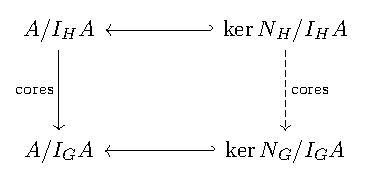
\includegraphics{lectures/6/pictures/cd_14.pdf}
	 \end{center}

	 и $\cores$ в $-1$-й размерности определяется как пунктирная стрелка, замыкающая эту диаграмму. Отметим, что эта стрелка есть, так как $G = \bigsqcup_{i} \sigma_i H$ и тогда
	 \[
	 	\sum_{h \in H} hx = 0 \implies \sum_{g \in G} gx = \sum_{i} \sigma_i \lr*{\sum_{h \in H} h x} = 0.
	 \]

	 Таким образом, мы распространили коограничение на $-1$-ю группу когомологий Тейта. 

	 Теперь распространим коограничение на положительные размерности. Это мы сделаем при помощи коиндуцированных модулей. Пусть $A^* = \Hom(\Z[G], A)$, рассмотрим диаграмму 
	 \[
	 	0 \to A \xrightarrow{i} A^* \to A' \to 0,
	 \]
	 где $i(a) = \varphi_{a}$, который действует так: $\varphi_a(g) = g^{-1}a$ (ясно, что отображение $i$ инъективно), а  $A' = \Coker{i}$. Тогда из длинной точной последовательности пары мы получаем (и того факта, что коиндуцированный модуль гомологически тривиален), что 
	\[
		\widehat{H}^{-1}(G, A') \cong \widehat{H}^0(G, A), \quad \widehat{H}^{-1}(H, A') \cong \widehat{H}^0(H, A). 	
	 \]

	 \begin{remark}
	 	Как и в предыдущем рассуждении такого толка тут также нужно проверить, что $A^*$ является не только $G$-коиндуцированным, но и $H$-коиндуцированным. 
	 \end{remark}

	 Итак, у нас есть диаграмма 

	 \begin{center}
	 	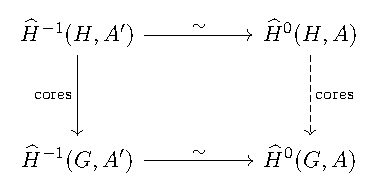
\includegraphics{lectures/6/pictures/cd_15.pdf}
	 \end{center} 

	 и $\mathrm{cores}$ в нулевой размерности мы определяем, как пунктирную стрелочку, замыкающую эту диаграмму. 


	 Теперь при помощи диаграммного поиска выпишем явную формулу для коограничения. Рассмотрим диаграмму 
	 \begin{center}
	 	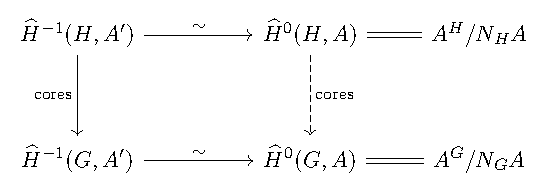
\includegraphics{lectures/6/pictures/cd_16.pdf}
	 \end{center}

	 Возьмём класс $\overline{\varphi} \in \widetilde{H}^{-1}(H, A') \cong \Ker{N_H}/I_{H}A' \subset A'/I_H A'$. Рассмотрим вот такую диаграмму: 

	 \begin{center}
	 	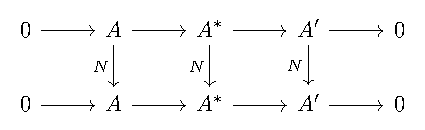
\includegraphics{lectures/6/pictures/cd_17.pdf}
	 \end{center}

	 Тогда $N_{H}\overline{\varphi} = 0 \implies N_H \varphi = \varphi_{a} \in A^*$, где $\varphi_a(g) = g^{-1}a$.  Пусть $G = \sqcup_{i} \sigma_i H$, тогда мы имеем такую диаграмму: 
	 \begin{center}
	 	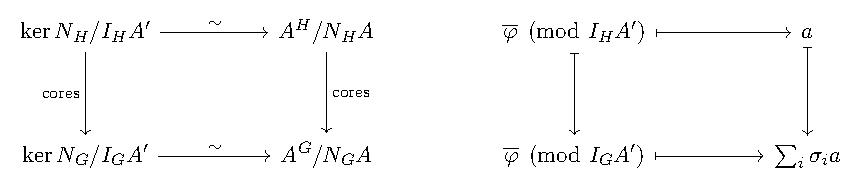
\includegraphics{lectures/6/pictures/cd_18.pdf}
	 \end{center}

	 Покажем, что $\overline{\varphi} \pmod{I_{G} A'} \mapsto \sum_{i} \sigma_i a$. Отметим сразу, что из этого будет следовать, что 
	 \[
	 	\cores^0(a) = \sum_{i} \sigma_i a.
	 \]

	 Теперь докажем требуемый факт. Он следует из нашего замечания выше о том, что $N_H \varphi = \varphi_a$:
	 \[
	 	(N_{G}\varphi)(g) = \lr*{\sum_{i}\sigma_i N_{H}\varphi}(g) = (\sum_{i}\sigma_i \varphi_a)(g) = \varphi_{\sum_i \sigma_i a}(g),
	 \]
	 что и требовалось. 

	 \subsection{Композиция ограничения и коограничения}

	 Теперь выведем из только что доказанной формулы для $\cores^0(a)$  полезные следствия. 

	 Пусть $G$~-- конечная группа, рассмотрим композицию
	 \[
		A^{G}/N_{G}A \xrightarrow{\res} A^H/N_{H}A \xrightarrow{\cores} A^{G}/N_{G}A	 	
	 \]

	 Соответственно, идя по композиции мы получаем
	 \[
	 	a \in A^{G} \mapsto a \in A^H \mapsto \sum_{i} \sigma_{i} a,
	 \]
	 но так как изначально $a \in A^G$, мы имеем $\forall i \ \sigma_i a = a$, откуда 
	 \[
	 	\cores(\res(a)) = [G : H] \cdot a.
	 \]

	 Аналогичные формулы можно получать и в больших размерностях при помощи сдвига (посредством длинной точной последовательности когомологий). 

	 Пусть $q \ge 1$, рассмотрим вновь короткую точную последовательность 
	 \[
	 	0 \to A \to A^* \to A' \to 0,
	 \]
	 где стрелка $A \to A'$ устроена как $a \mapsto \varphi_a, \ \varphi_a(g) = g^{-1}a$, а $A'$~--- это коядро этой стрелки. 

	 Соответственно, так как для $q \ge 1$ когомологии с коэффициентами в $A^*$ тривиальны, из длинной точной последовательности когомологий мы можем заключить, что $H^{q - 1}(G, A') \cong H^{q}(G, A)$ (т.е. мы можем сдвинуть размерность). Теперь рассмотрим диаграмму: 

	 \begin{center}
	 	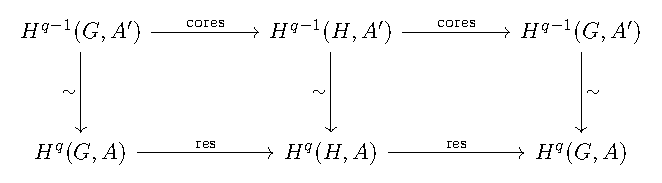
\includegraphics{lectures/6/pictures/cd_19.pdf}
	 \end{center}

	 Коммутативность правого квадрата следует из определения $\cores^q$, а коммутативность левого квадрата следует из того, что связывающий гомоморфизм коммутирует с гомоморфизмами точных троек комплексов. 

	 Предположим, что мы доказали требуемую формулу для $q - 1$ (т.е. для верхней строчки диаграммы). Тогда по индукционному предположению мы имеем 
	 \[
	 	\cores^{q - 1} \circ \res^{q - 1}(a) = [G : H] \cdot a,
	 \]
	 и из коммутативности диаграммы отсюда мы можем заключить, что утверждение верно и для $q$. 


	 Теперь коротко обсудим, что же происходит в отрицательной размерности. Как нетрудно догадаться, там нужно рассмотреть короткую точную последовательность 
	 \[
	 	0 \to A'' \to A_* \to A \to 0
	 \]
	 и воспользоваться тем, что для групп отрицательной размерности когомологии с коэффициентами в модуле $A_*$ тривиальны, а тогда из длинной точной последовательности пары мы заключаем, что 
	 \[
	 	\widehat{H}^q(G, A) \cong \widehat{H}^{q - 1}(G, A''),
	 \]
	 откуда следует, что можно делать сдвиг размерности влево. 

	 Итого, в этом параграфе мы доказали такую теорему: 

	 \begin{theorem} 
	 	Пусть $G$~--- конечная группа, $H \le G$~--- подгруппа. Тогда во всех размерностях выполнена такая формула: 
	 	\[
	 		\cores \circ \res(a) = [G : H] \cdot a.
	 	\]
	 \end{theorem}

	 \begin{corollary}
	 	Если $H = e$~--- тривиальная подгруппа, то $\res = 0$ (так как $H^{\bullet}(H, A) = 0$),  и тогда мы (достаточно внезапно) имеем 
	 	\[
	 	 		|G| \cdot \widehat{H}^{q}(G, A) = 0,
 		\] 		
 		что говорит нам, что для конечных групп группы Тейта периодичны. Или же, что всякий коцикл, умноженный на порядок группы является кограницей. 
	 \end{corollary}

    Теперь поговорим про Силовские подгруппы. Пусть $p$~--- простое число, $S$~--- Силовская $p$-подгруппа в $G$. 

	 \begin{corollary}
	 	Отображение ограничения $\widehat{H}^q(G, A) \xrightarrow{\res} H^{q}(S, A)$~--- мономорфизм на $p$-примарной компоненте $\widehat{H}^q(G, A)$.  
	 \end{corollary}
	 \begin{proof}
	 	Пусть $|G| = p^{\alpha}m$, $(p^{\alpha}, m) = 1$ и пусть $x$ лежит в $p$-примарной компоненте $\widehat{H}^q(G, A)$. Предположим, что $\res(x) = 0$. Тогда 
	 	\[
	 		0 = \cores \circ \res(x) = [G : S] \cdot x
	 	\]
	 	Таким робразом, $p^{\alpha} x = 0$ и $m x = 0$, а так как $(p^{\alpha}, m) = 1$, отсюда мы имеем, что $x = 0$. 
	 \end{proof}

	 \begin{corollary}\label{Sylow_subgroups_mono}
	 	Отображение $\widehat{H}^q \xrightarrow{\bigoplus \res_{G/S_p}} \bigoplus_{p} \widehat{H}^{q}(S_p, A)$~--- мономорфизм (тут $S_p$ пробегает все Силовские $p$-подгруппы).
	 \end{corollary}
	 





